%%%%%%%%%%%%%%%%%%%%%%%%%%%%%%%%%%%%%%%%%%%%%%%%%%%%%%%%%%%%%%%%%%%%%%%%%%%%%%%%
% Diese Datei beinhaltet den eigentlichen Inhalt Ihrer Arbeit.
%
% Es bietet sich der Übersicht halber an, die einzelnen Abschnitte jeweils
% in eigene Dateien zu schreiben und mittels \input einzubinden.
% Eine mögliche Verzeichnisstruktur sähe entsprechend so aus:
%
%     thesis/
%     +- tex/
%     |  +- introduction.tex
%     |  +- motivation.tex
%     |  +- experiments.tex
%     |  |  ...
%     |  +- conclusion.tex
%     +- abstract.tex
%     +- contents.tex
%     +- thesis.tex
%%%%%%%%%%%%%%%%%%%%%%%%%%%%%%%%%%%%%%%%%%%%%%%%%%%%%%%%%%%%%%%%%%%%%%%%%%%%%%%%

\section{Einleitung}

Dies ist der Hauptteil Ihrer Arbeit.
In der Datei \texttt{references.bib} finden Sie bereits einige Quellen,
die Sie wahrscheinlich zitieren mögen,
wie z.B. die B Methode~\cite{abrial1996b,abrial2010modeling}
oder \textsc{ProB}~\cite{leuschel2003prob,leuschel2008prob}.
Beachten Sie den Artikel ``Common Errors in Bibliographies'' von John Owens.%
\footnote{\url{https://www.ece.ucdavis.edu/~jowens/biberrors.html}}

\cref{sec:figures,sec:tables}
geben je ein kurzes Beispiel,
wie Bilder bzw. Tabellen in \LaTeX{} erstellt werden.
\cref{sec:plot} zeigt die Einbindung eines Graphen.


\subsection{Makefile}

Im Wurzelverzeichnis finden Sie ein \texttt{Makefile}.
Über das Terminal können Sie die folgenden Befehle aufrufen:


\begin{tabularx}{\textwidth}{lX}
  \toprule
  \texttt{make} & Kompiliert das PDF und löscht aux-Files. \\
  \texttt{make clean} & Löscht das PDF und dazugehörige aux-Files. \\
  \texttt{make bibtool} & Sortiert \texttt{references.bib}
  und formatiert die Einträge einheitlich. \\
  \texttt{make watch} & Rekompiliert das PDF bei Änderungen und
  hält die Anzeige in Ihrem PDF-Betrachter aktuell. \\
  \bottomrule
\end{tabularx}

\section{Bilder und Co.}

\subsection{Bilder}%
\label{sec:figures}

\begin{figure}[h]
  
\includegraphics[width=4cm]{fig/the.png}
  \caption{Initial thesis draft.}%
  \label{fig:initial-draft}
\end{figure}

In \cref{fig:initial-draft} ist festgehalten,
wie alles angefangen hat.


\subsection{Tabellen}%
\label{sec:tables}

\cref{table:truths} fasst die Wahrheiten dieser Welt zusammen.

\begin{table}[ht]
  \begin{center}
    \begin{tabular}{lr}
      \toprule
      Fakt                                & Wahrheitsgehalt \\
      \midrule
      booktabs Tabellen sind hübscher     & 90 \%           \\
      Han Solo schoss zuerst              & 100 \%          \\
      Game of Thrones fand ein gutes Ende & 0 \%            \\
      \bottomrule
    \end{tabular}
    \caption{Table of truths.}%
    \label{table:truths}
  \end{center}
\end{table}

\subsection{Plots}%
\label{sec:plot}

Sie können mithilfe von \texttt{tikz} und \texttt{pgfplots}
ganz leicht Graphen erstellen:

\begin{figure}[ht]
  \centering
  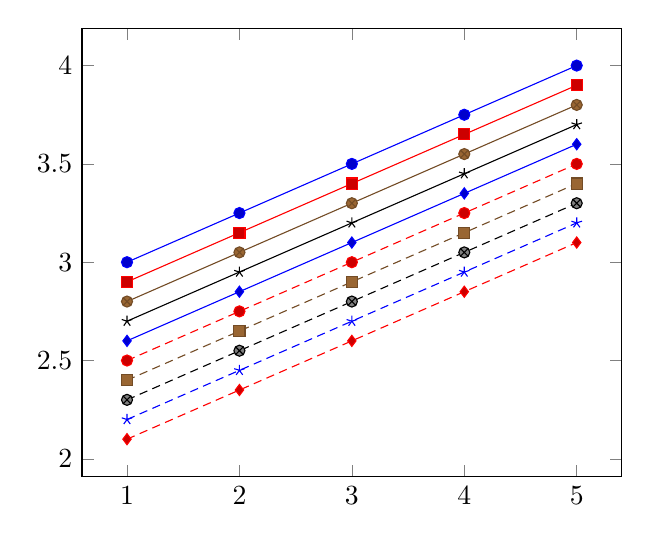
\begin{tikzpicture}
    \begin{axis}
      \foreach \y in {0,0.1,...,1} % Wiederholt \addplot mit jeweils anderem \y
        \addplot coordinates {
            ( 1, 3.0 -\y)
            ( 2, 3.25-\y)
            ( 3, 3.5 -\y)
            ( 4, 3.75-\y)
            ( 5, 4.0 -\y)
          };
    \end{axis}
  \end{tikzpicture}
  \caption{A beautiful plot.}%
  \label{fig:the-plot}
\end{figure}

\section{Conclusion}

Am Ende der Arbeit werden noch einmal die erreichten Ergebnisse
zusammengefasst und diskutiert.
